\chapter{Preliminaries}

\section{Sounding Rockets}
A sounding rocket is designed to carry scientific payloads and experiments in a suborbital flight profile. The altitude at apogee of sounding rockets varies greatly. As an example, sounding rockets designed by \gls{nasa} can reach altitudes from 50\,km to 1300\,km, while students build high power rockets often only go up to 10\,km. The rocket and, in some cases, only the payload gets recovered by a parachute system. These systems always consist of multiple parachute stages to minimize drift from the launch site.\cite{nasa-rockets}

\begin{figure}[h!]
	\centering
	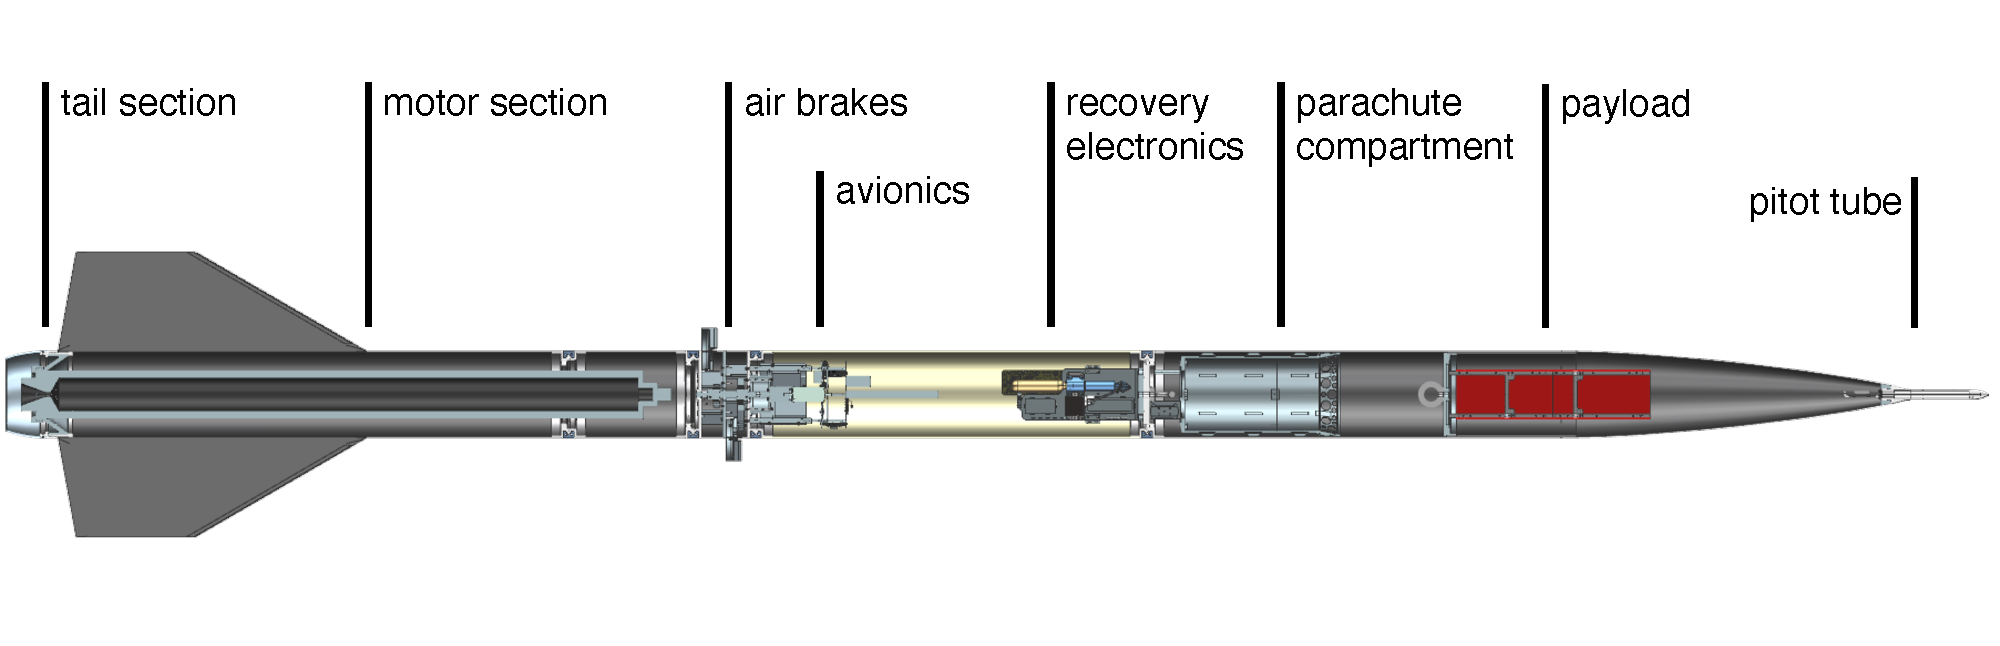
\includegraphics[width=\textwidth]{images/EULER_FSL_CAD}
	\caption{CAD drawing of the rocket EULER from ARIS}
	\caption*{\textbf{Source:} ARIS EULER 2021 EuRoC Report \cite{euler-euroc_report}}
	\label{fig:euler}
\end{figure}

The rocket in Figure \ref{fig:euler} was developed by \acrshort{aris} members for the \acrfull{euroc} in Portugal. It is equipped with an air breaks system to accurately hit a target apogee, an avionics system to transmit telemetry data, and a custom-developed recovery system. The parachute system consists of a drogue and main chute, and a scientific payload can be carried and recovered. The rocket has a dry mass of almost 40\,kg and is 4.2\,m long.  


\newpage

\subsection{Concept of Operation}\label{conops}
Sounding rocket operations are often separated into the phases shown in Figure \ref{fig:operation}.

\begin{figure}[h!]
	\centering
	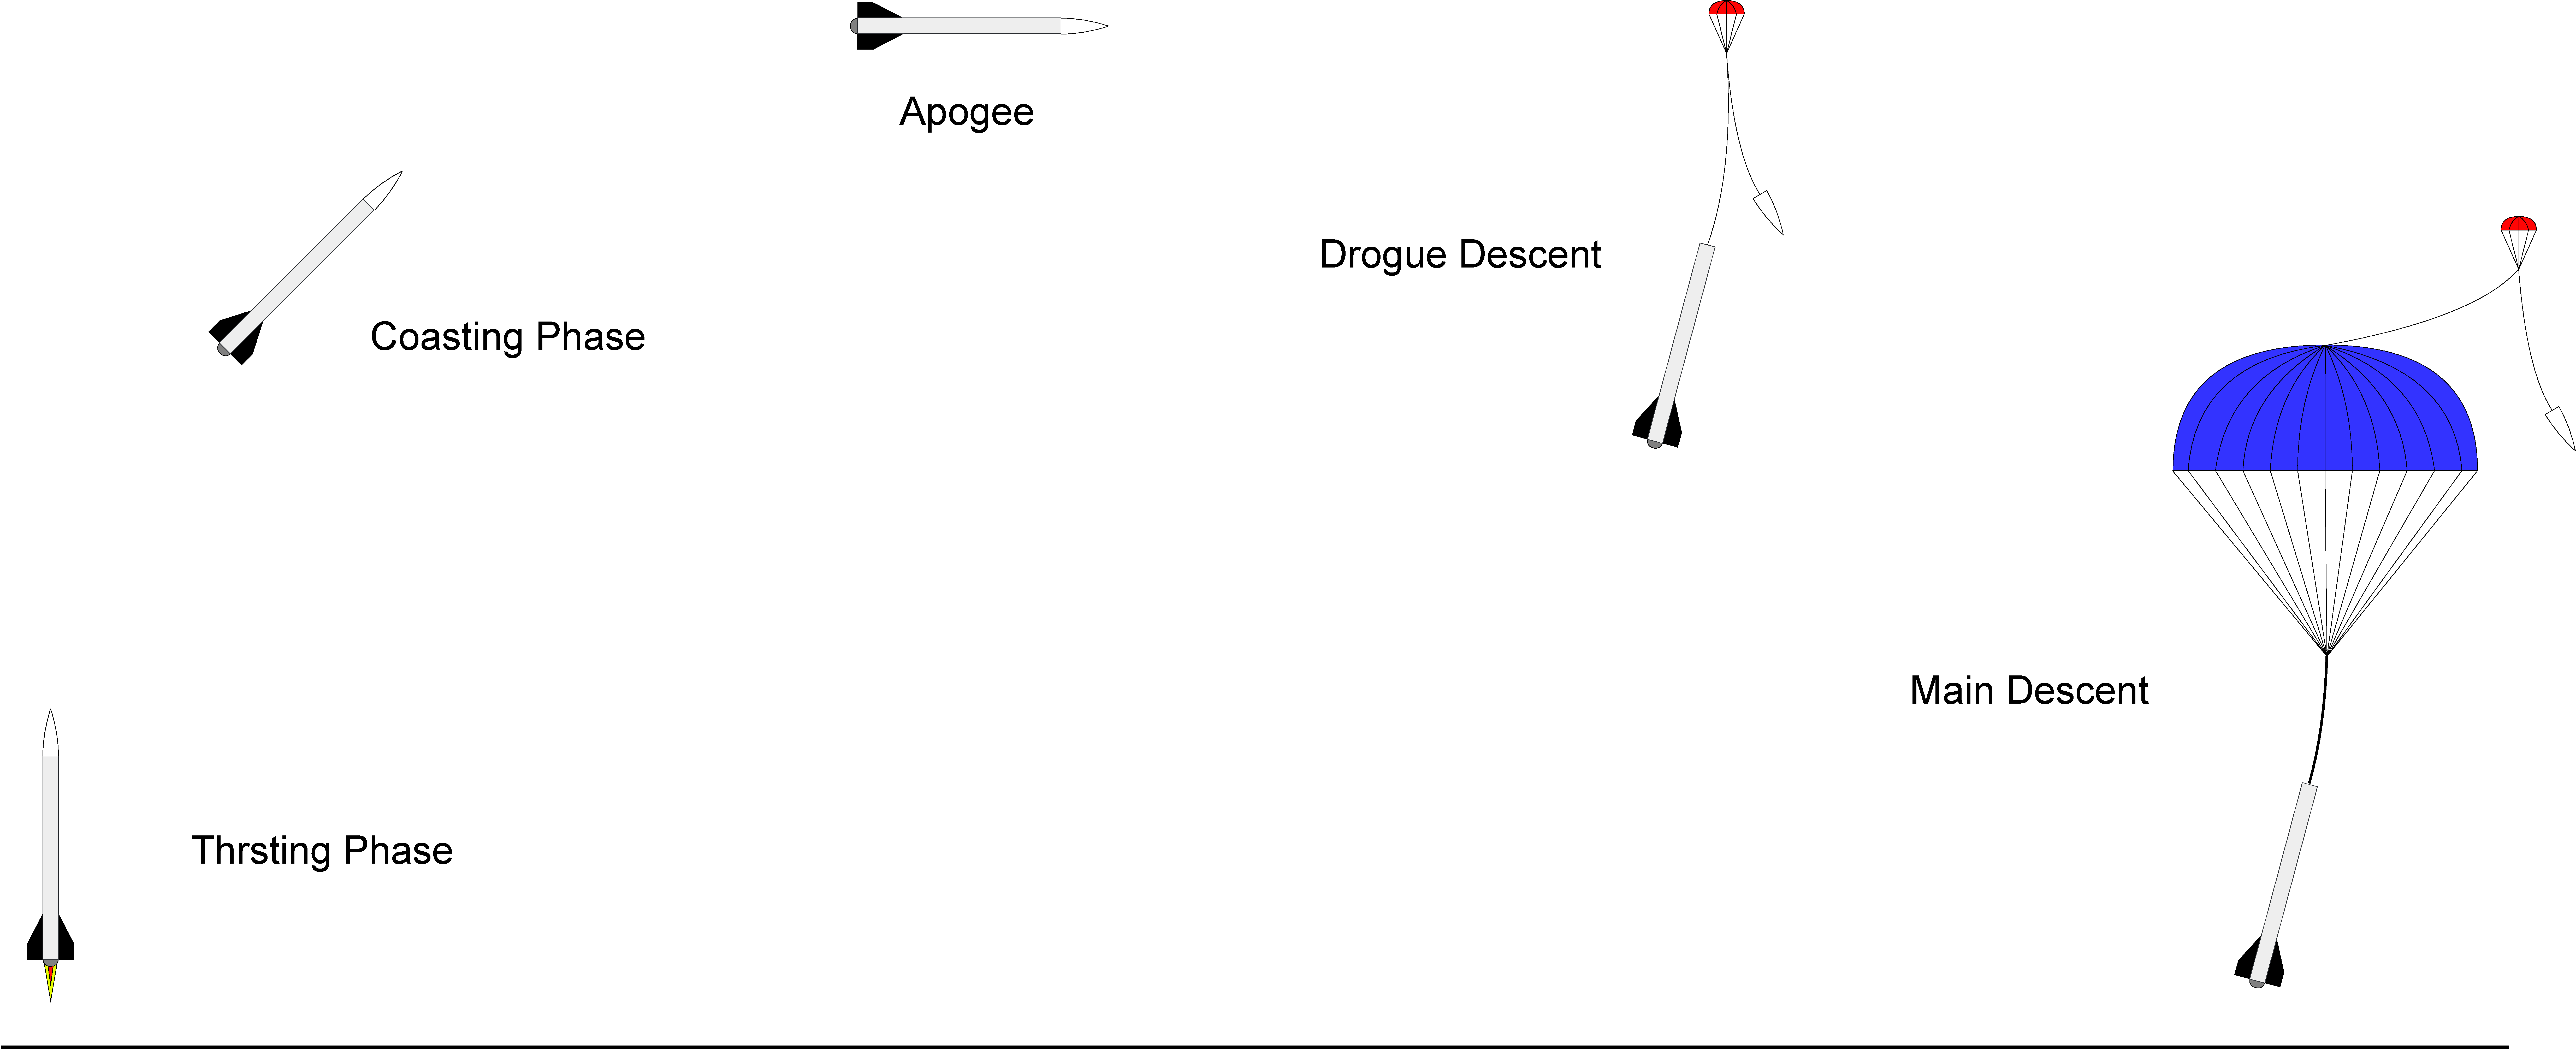
\includegraphics[width=\textwidth]{images/rocket-operation}
	\caption{Illustration of rocket operation}
	\label{fig:operation}
\end{figure}

\subsubsection{Thrusting Phase}
The rocket begins its flight without support from the launch rail and accelerates until the motor burns out. During this phase, accelerations can reach incredibly high numbers, depending on the flight profile. For example, the rockets from the association \acrshort{aris} usually accelerate at around 20\,g but accelerations as high as 100\,g can be experienced. The maximum velocity is reached just at the point of burnout.

\subsubsection{Coasting Phase}
Starting with burnout of the motor, the rocket enters the coast phase. Drag and gravitational forces cause the rocket to decelerate until it reaches apogee. At altitudes above 80\,km, aerodynamic forces are almost nonexistent, leaving the payload exposed to a microgravity environment.

\subsubsection{Drogue Descent}
The drogue parachute sends the rocket into a stable descent to allow a reliable deployment of the main parachute. Drogue parachute deployment causes shock forces to be applied to the rocket structure. For structural reasons, the drogue is often deployed at apogee, where the rocket's velocity is at its lowest point of the flight.

\subsubsection{Main Descent}
In order to minimize the velocity before ground impact, a larger main parachute is deployed close to the ground. The shock loads during the parachute opening are the highest the rocket will experience during its flight. To minimize these forces, a gradual opening of the parachute is preferred.

\newpage

\section{Parachute Reefing}
Parachute reefing permits the gradual opening of the parachute canopy or restricts its full inflation or overinflation. Advantages of parachute reefing include:
\begin{itemize}
		\item Reducing the parachute opening forces. 
		\item Obtain a temporarily high rate of descent. Reefing the parachute to a low drag area permits a more accurate descent from a high altitude. Low-impact velocity is then obtained by disreefing the parachute shortly before ground impact. 
		\item Increase parachute stability by a slight amount of fixed reefing.
\end{itemize}
Two reefing methods are discussed in the following subsections.\cite[Chapter~5.6]{parachute-design}

\subsection{Skirt Reefing}
Skirt reefing is the most commonly used reefing method. 

Reefing rings are located at the connection points of each suspension line inside the canopy skirt. Reefing lines, which are continuous ropes that prevent the canopy from opening, are guided through the reefing rings and several reefing line cutters. Upon firing the cutter at the preset time, it cuts off the reefing line, allowing the canopy to open up or advance to the next stage.

Multiple reefing stages can be added to reduce the forces between each stage.\cite[Chapter~5.6]{parachute-design}

\begin{figure}[h!]
	\centering
	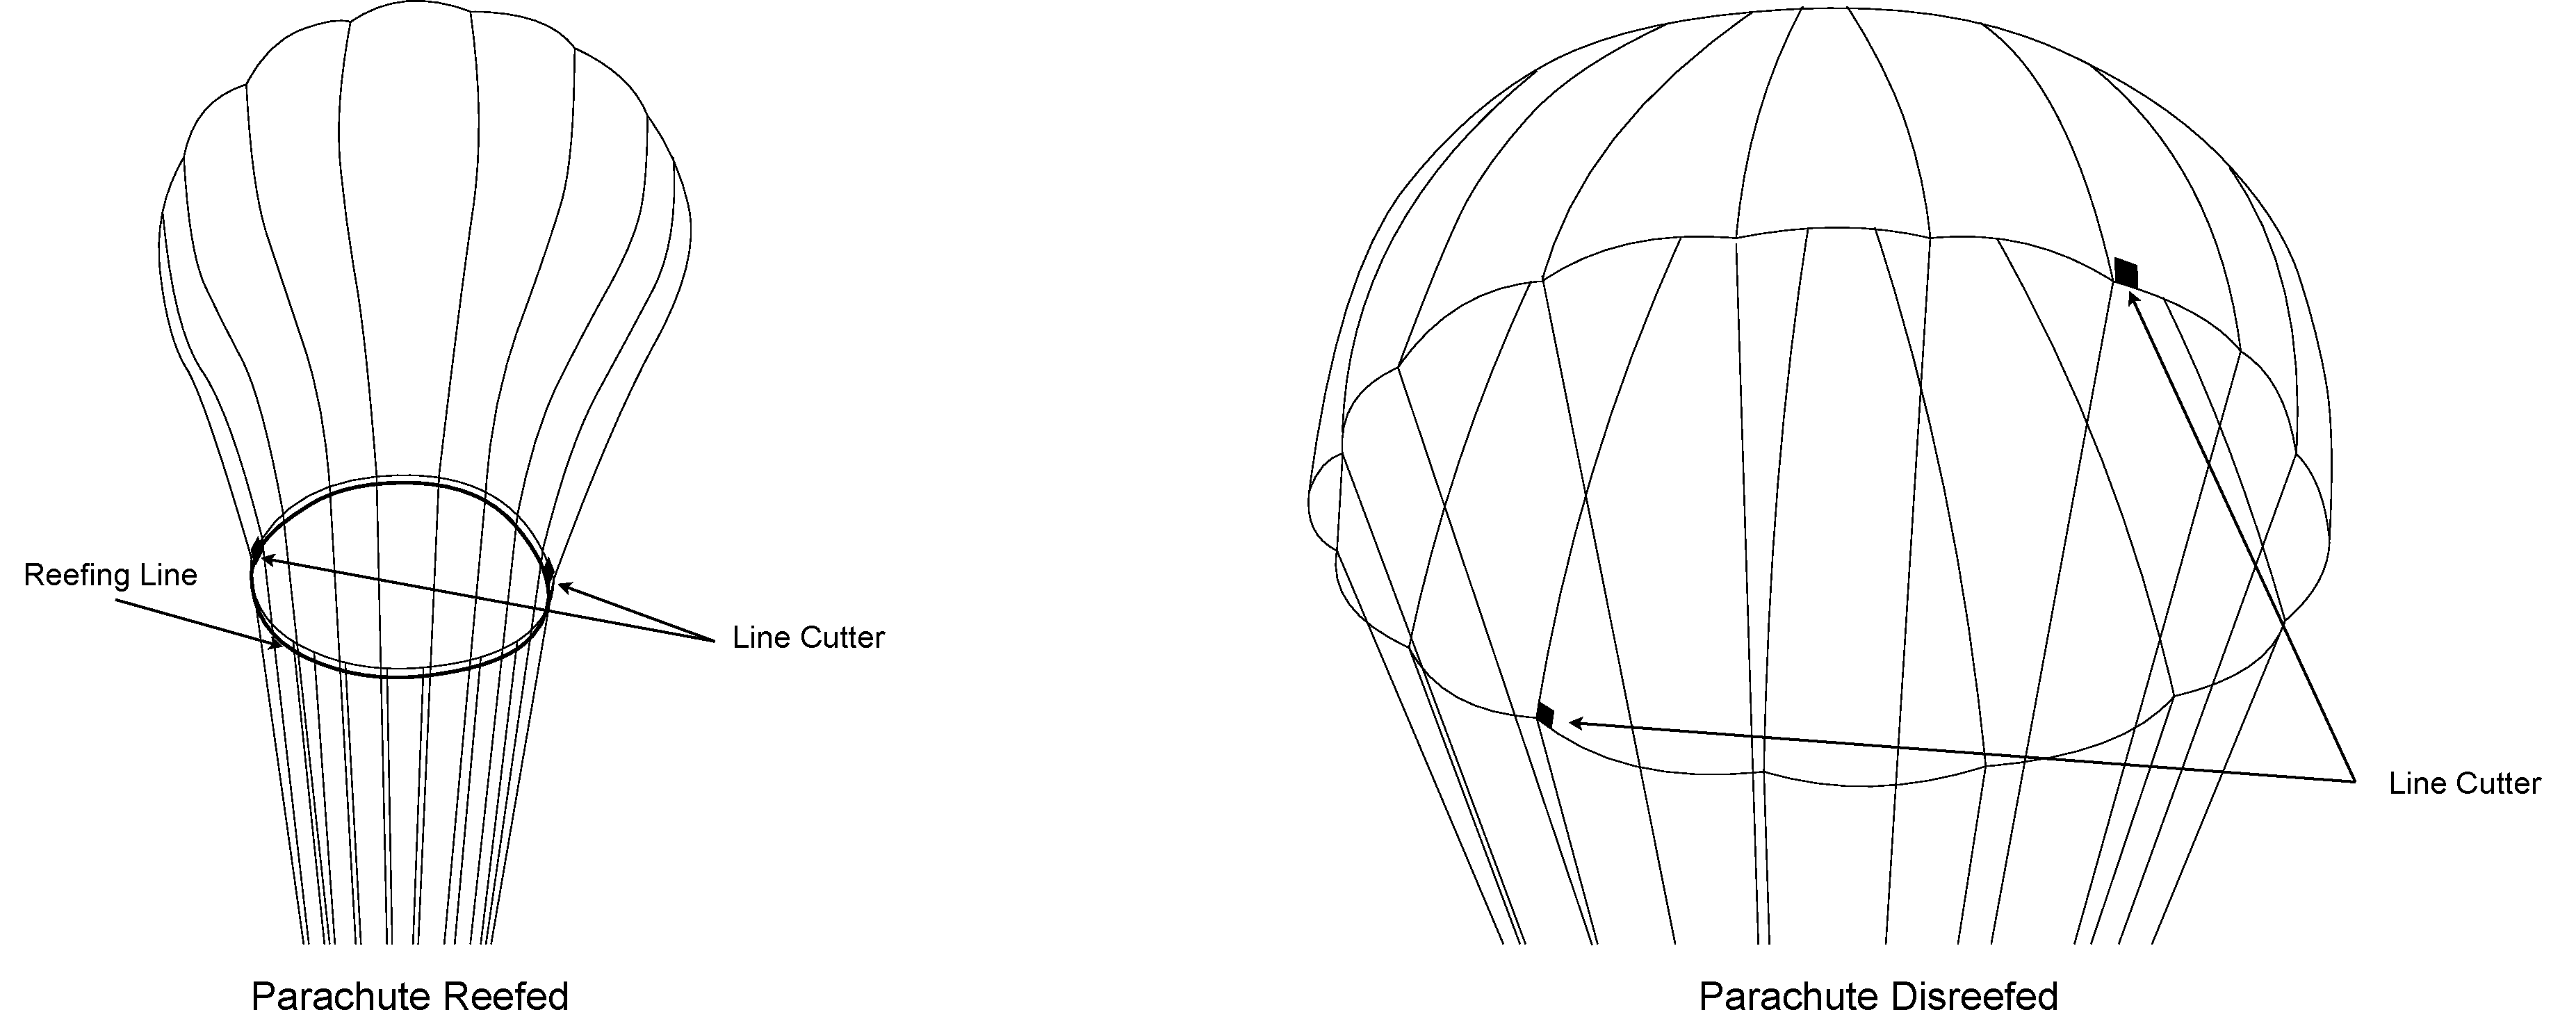
\includegraphics[width=\textwidth]{images/reefing-iilustration}
	\caption{Illustration of skirt reefing system}
	\label{fig:reefing-iilustration}
\end{figure}

\subsection{Continuous Disreefing}
A reefing system in which a pre-selected force-time diagram governs the opening of the parachute canopy is considered the pinnacle of reefing systems. Many attempts have been made to develop such a system. However, none of these attempts resulted in a practical solution.\cite[Chapter~5.6]{parachute-design}

\newpage

\section{Wireless Transmission Methods}

\subsection{Chirp spread spectrum}
\acrfull{css} is a modulation technique used in wireless transmission. It uses its entire allocated bandwidth for broadcast, making it robust to channel noise. The data transmission is based on chirps; a chirp is a sinusoidal signal that linearly increases or decreases in frequency over time. Symbols can be encoded by varying the start frequency as shown in Figure \ref{fig:css}.\cite{css-wiki}

\begin{figure}[h!]
	\centering
	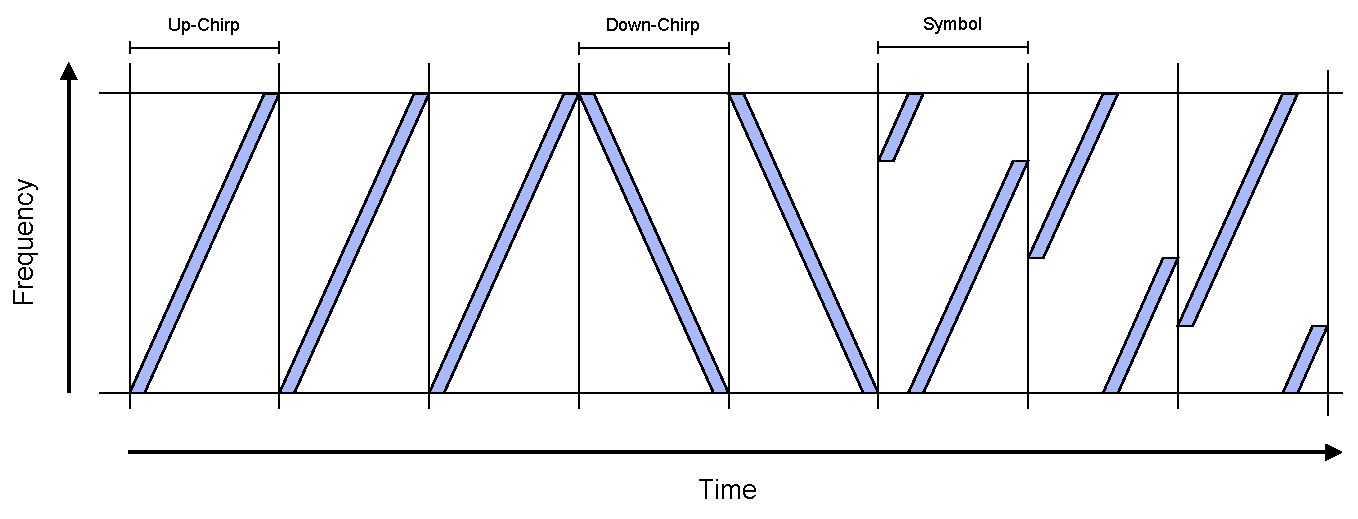
\includegraphics[width=\textwidth]{images/css}
	\caption{\acrshort{css} transmission example}
	\label{fig:css}
\end{figure}

\subsubsection{LoRa}
\acrshort{lora} is a physical proprietary radio modulation technique developed by Cycleo, which Semtech later acquired. \acrfull{css} modulation is used for the transmission. The technology is ideal for applications that transmit small chunks of data with low bit rates. Compared with Wi-Fi, Bluetooth, or ZigBee, data can be transmitted over a longer distance. As a result of these features, \acrshort{lora} is well suited for sensor nodes that operate on a limited power budget.\cite{lora-ttn}

\acrshort{lora} can be operated on the license-free sub-gigahertz bands, such as 915 MHz, 868 MHz, and 433 MHz. It can also work at 2.4 GHz, which achieves higher data rates than sub-gigahertz bands at the expense of range. The frequencies in question are within the ISM bands, reserved internationally for industrial, scientific, and medical uses. \cite{ism-wiki}

The name, \acrshort{lora}, is a reference to the extremely long-range data links that this technology enables. 

\newpage

\subsection{Frequency Hopping Spread Spectrum}
\acrfull{fhss} is a method of transmitting radio signals over rapidly changing carrier frequencies. The frequency band is subdivided into narrow channels. Throughout these channels, signals change their carrier frequencies rapidly in a predetermined order. The transmission requires both the transmitter and receiver to know the hopping pattern. A key benefit of \acrshort{fhss} is that it makes transmissions much more resistant to interference and more difficult to intercept. Allowing more devices on the same frequency band with little or no impact on the link quality.\cite{fhss-wiki}

\begin{figure}[h!]
	\centering
	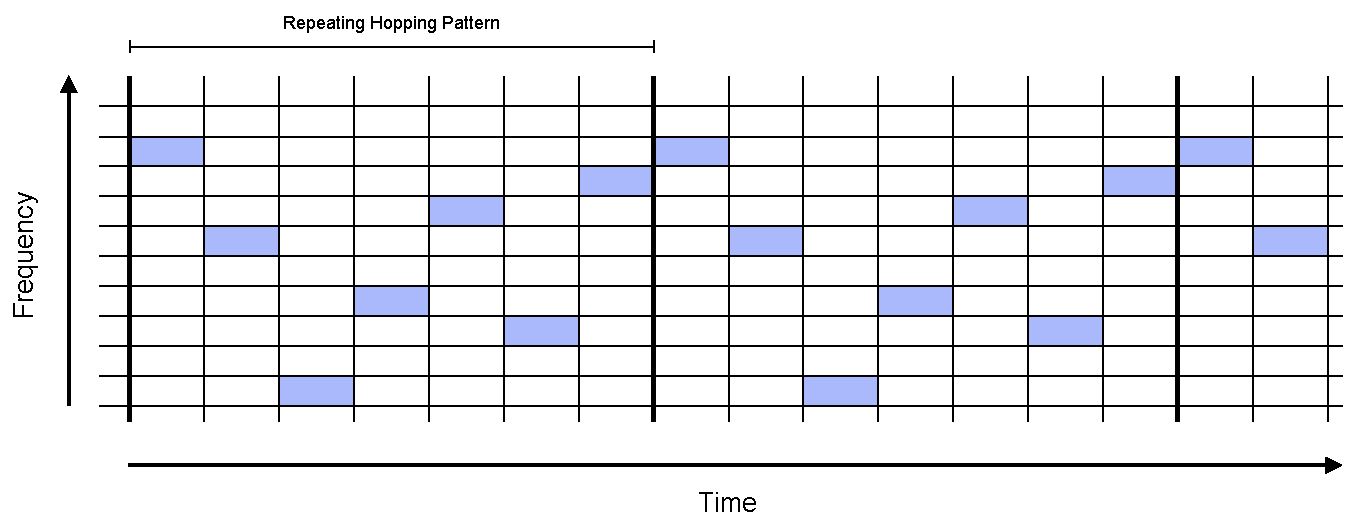
\includegraphics[width=\textwidth]{images/fhss}
	\caption{\acrshort{fhss} transmission example}
	\label{fig:fhss}
\end{figure}

As shown in Figure \ref{fig:fhss}, the frequency is changed with a fixed interval. One of the challenges when developing a \acrshort{fhss} protocol is the synchronization of the transmitter and receiver. The receiver needs to wait for a package to be received. Also, when no data is received, it needs to switch to the subsequent frequency in time. Therefore the time synchronization between the devices is critical. 
\newpage

\section{Kalman Filter}
Kalman filters are used to estimate states based on linear dynamical systems. Using a series of measurements observed over time, including statistical noise and other inaccuracies, the algorithm produces estimates of unknown variables that are usually more accurate than those based solely on a single measurement.

The filter was developed by Rudolf E. Kálmán, after whom the algorithm is named. Although Thorvald Nicolai Thiele and Peter Swerling developed a similar algorithm earlier.\cite{kalman-wiki}

\subsection{Kalman Filter Model}
A Kalman filter is typically built in two phases. A prediction advances the state until the following scheduled observation, while the update step incorporates that observation. It is, however, not necessary for the filter to have two phases. If an observation is not available, the update may be skipped and multiple prediction steps performed. In the same way, if there are several independent observations, multiple updates may be performed as well.\cite{kalman-introduction}

The Kalman Filter model assumes the true state $x_k$ at time ${k}$ from the previous state ${k-1}$. Thus the process model is defined according to
\begin{equation}
    x_{k} = Ax_{k-1} + Bu_{k} + w_{k}
\end{equation}
where
\begin{itemize}
    \item $A$ is the state transition model applied to the previous state $(x-1)$;
    \item $B$ is the control input model applied to the control vector $u_k$;
    \item $w_k$ is the process noise, which is assumed to be a zero mean normal distribution $\mathcal{N} (0, \sigma)$.
\end{itemize}

The measurement model describes the relationship between the state and the measurement at current time $k$. The model takes an observation of the true state  
\begin{equation}
    z_{k} = Cx_{k} + v_{k}
\end{equation}
where
\begin{itemize}
    \item $C$ is the observation model, which maps the true state into the observation state;
    \item $v_k$ is the observation noise, which is assumed to be a zero mean normal distribution $\mathcal{N} (0, \sigma_R)$.
\end{itemize}
